% Methods
\section{Methods}

\begin{figure}
  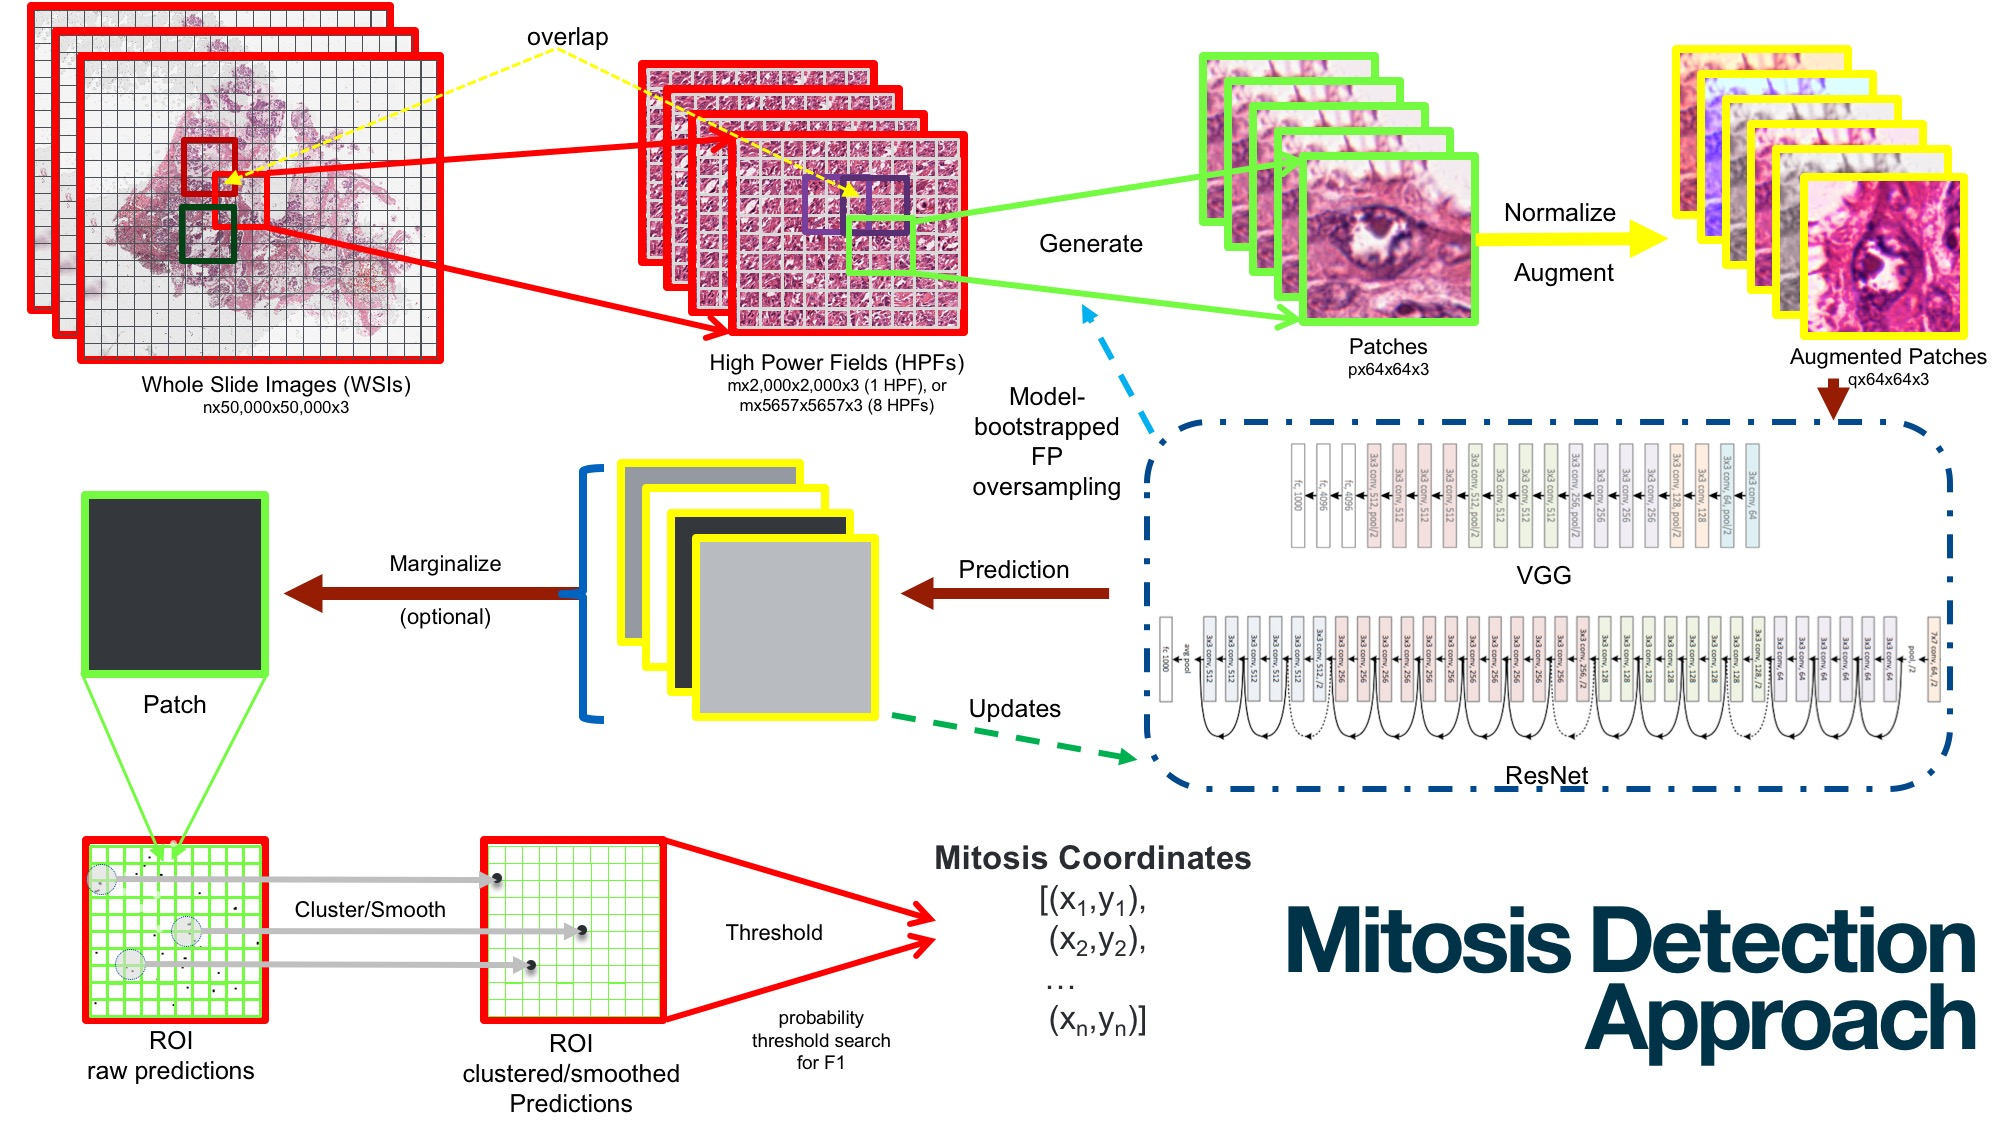
\includegraphics[width=\linewidth]{assets/diagram}
  \caption{Mitosis detection approach.}
  \label{fig:approach}
\end{figure}

At a high level, as shown in  Figure \ref{fig:approach}, our approach begins by preprocessing a dataset of regions of tissue from \glspl{wsi} of breast tumors into a dataset of mitotic and non-mitotic patches.  We then train a \gls{conv} model to predict the presence of a mitotic figure in a given patch.  Given an initial trained model, we preprocess the raw dataset again with model-based \gls{fp} oversampling to generate a more difficult training dataset.  We then train a new model on this second dataset.  To make predictions on a new image region, we apply the model to the image in a sliding window fashion with noise marginalization, yielding a prediction at each location.  A clustering algorithm is then used to smooth the potentially noisy set of predictions into a set of final predictions for mitosis locations.

\paragraph{Preprocessing}
\label{par:prep}
We begin with a dataset of breast cancer cases, in which each case contains images of regions of tissue extracted from \glspl{wsi} of breast tumors and accompanying exhaustive lists of $(x,y)$ coordinates corresponding to the center of each mitotic figure.  The dataset is randomly split case-wise into training and validation sets, stratified by lab of origin, if available, and constrained to include some percentage of the cases in the training set.  We then generate training and validation datasets of mitotic and non-mitotic square image patches in which each side is of length $l_\text{prep}$.  Mitotic patches are extracted from locations centered at the given labeled coordinates.  Non-mitotic patches are extracted in a sliding window fashion with a stride $s_\text{prep}$, and are constrained to be at least $2d$ pixels in Euclidean distance apart from the center of each mitotic figure. Additionally, we sample from the set of all potential non-mitotic patches by drawing, for each patch, a decision from a Bernoulli distribution governed by a parameter $p$.


\paragraph{Training}
Given our preprocessed data, our training algorithm proceeds as follows.  First, we randomly shuffle the training set, augment and normalize each example, and generate batches of size $n_\text{train}$ examples by sampling from the training set, possibly with oversampling of the minority mitosis class.  Our data augmentation algorithm includes a random rotation; a random translation via random cropping to a square with sides of length $l_\text{train}$ such that the center is within $d-5$ pixels in Euclidean distance from the original center; random flips along the spatial axes; and color augmentation instead of color normalization \cite{Macenko:2009hf}.  Our color augmentation approach uses parameterized random brightness, contrast, saturation, and hue adjustments, with values based on recent work \cite{Liu:2017uu}.  We normalize each example to the interval $[-1,1]$.  Minority oversampling via class-aware sampling \cite{Shen:2016uo} is used to yield balanced batches, and we define an epoch as the number of batches needed to exhaust the list of non-mitotic patches.  Minority oversampling has been shown to be an effective approach to improve classification performance of \glspl{conv} in class-imbalanced problems \cite{Buda:2017tg}.
%Minority oversampling has been shown to be an effective approach to improve classification performance of \glspl{conv} in class-imbalanced problems \cite{Buda:2017tg}.  Our approach employs minority oversampling via class-aware sampling \cite{Shen:2016uo} to yield balanced batches, defining an epoch as the number of batches needed to exhaust the list of non-mitotic patches.

Our first model is a modified \gls{resnet} \cite{He:2015tt}, specifically a \gls{resnet}-50, with pretrained weights\footnote{\url{https://www.tensorflow.org/versions/master/api_docs/python/tf/keras/applications/ResNet50}}.  We replace the final affine and softmax functions with a new binary affine function and a sigmoid function, update the stride on the first convolution layer from $2 \times 2$ to $1 \times 1$ for ``$\text{height} \times \text{width}$", and update the final average pooling function to a kernel size of $4 \times 4$.

Our second model is a custom \gls{resnet} using the updated residual block formulation \cite{He:2016tq} with bottlenecks.  The model contains an input block, three groups or ``stages" of three residual blocks each, and an output block.  The input block has a single 2D convolution function with a kernel of shape $(3, 3, 3, 16)$ for (height, width, input depth, output depth), $2\times 2$ stride, and appropriate spatial padding such that the output tensor has the same height and width as the input tensor, i.e., ``same" padding.  The first ``stage" is defined as a set of three residual blocks with $3 \times 3$ kernels and $1\times 1$ strides, where the output kernel depth is 32.  The second and third stages are each defined as a residual block with a $3\times 3$ kernel and $2\times 2$ stride, followed by two residual blocks with $3\times 3$ kernels and $1\times 1$ strides.  The output kernel depth of the second stage is 64, and that of the third stage is 128.  The output block has a batch normalization function \cite{Ioffe:2015ud}, a ReLU function \cite{Nair:2010vq}, a global average pooling function \cite{Lin:2013wb}, an affine function to yield a single output value per example, and a sigmoid function.  All convolution function parameters are initialized by sampling from a standard Gaussian distribution scaled by $\sqrt{\frac{2}{D}}$ \cite{He:2015vx}, where $D$ is the number of values in a single example of the input tensor for the given function, and the final affine function parameters are initialized by sampling from a standard Gaussian distribution scaled by $\sqrt{\frac{1}{D}}$ \cite{LeCun:1998dl}.  All batch normalization functions use a momentum of $0.9$ and an epsilon term of $1\mathrm{e}{-4}$.
% include pre-trained models?

We use the logistic loss function, assuming a Bernoulli distribution parameterized by the model for each prediction.  Additionally, we add an L2 regularization term to the loss with a regularization parameter $\lambda$, assuming a standard Gaussian prior on all model parameters.  We employ transfer learning to train the first model by first optimizing the loss with respect to the parameters of the new affine layer for $e_1$ epochs using the Adam optimizer \cite{Kingma:2015us} with $\beta_1 = 0.9$, $\beta_2 = 0.999$, $\epsilon = 1\mathrm{e}{-8}$, and a learning rate $lr_1$.  Following that, we optimize the loss with respect to all model parameters for $e_2$ epochs using stochastic gradient descent with Nesterov momentum \cite{Bengio:2013tc}, with momentum $\mu$, and learning rate $lr_2$.  We train the second model by optimizing the loss with respect to all model parameters for $e$ epochs using the Adam optimizer with $\beta_1 = 0.9$, $\beta_2 = 0.999$, $\epsilon = 1\mathrm{e}{-8}$, and a learning rate $lr$.

Training proceeds by optimizing the loss for some number of epochs $e$.  At the end of each epoch, we evaluate the model on the training and validation preprocessed datasets, and save a checkpoint.  Evaluation metrics include \gls{ppv} (i.e., precision), sensitivity (i.e., recall),
%F1 score at threshold $0.5$,
 and maximum F1 score.  The best model is selected as the checkpoint that has the largest maximum F1 score on the preprocessed validation dataset.
%Due to the class imbalance, accuracy is a poor metric of choice.
%Hyperparameters are optimized through random grid search.


%\paragraph{Evaluation}
%Mean loss, accuracy, positive predictive value (i.e., precision), sensitivity (i.e., recall), F1 score at threshold $0.5$, and maximum F1 score are evaluated for both training and validation preprocessed datasets at the end of each epoch.


%\paragraph{Model Selection}
%The best model is selected as the checkpoint that has the largest maximum F1 score on the preprocessed validation dataset.


\paragraph{\Acrlong{fp} Oversampling}
The best \acrshort{resnet}-50 model trained on the initial preprocessed training dataset will exhibit a poor F1 score due to a low precision.  Motivated by work by \citet{Ciresan:2013hm}, we use the initial best model to generate a new intermediate preprocessed training dataset composed only of \gls{fp} cases.  A \gls{fp} case is defined as a candidate non-mitotic patch that is predicted as mitotic by the model.  Candidate non-mitotic patches are sampled following the preprocessing procedure outlined on page \pageref{par:prep}.  These non-mitotic \gls{fp} patches are then combined with the original preprocessed training dataset to yield a new model-bootstrapped preprocessed training dataset in which \gls{fp} cases have been oversampled.  The validation dataset remains the same to allow for proper comparisons.  Collectively, this new dataset is used to train the custom \gls{resnet} model.


\paragraph{Prediction}
% marginalization
% stride
% clustering
% detection
In order to make predictions of the locations of mitotic figures on the original raw dataset, we proceed as follows.  We first apply the best trained model to the original images in a sliding window fashion with a stride $s_\text{pred}$.  At each location, we either record the output of the model applied to a centered patch, or we apply noise marginalization and record the ensuing output.  Noise marginalization acts as a complement to data augmentation, where the latter injects noise $\eta$ during the training process to model $p(y|x,\eta)$, and the former marginalizes over the noise at test time to model $p(y|x) = \int p(y|x,\eta) d\eta$.  In practice, for each location we form a batch of $n_\text{pred}$ data-augmented variants of the centered patch, apply the model to this batch, and average over the batch of predictions to yield a single noise-marginalized prediction for the given location.

Evaluation of location predictions proceeds by defining a \gls{tp} as a ground-truth mitosis for which there exists at least one prediction within $d$ pixels in Euclidean distance from the mitosis; a \gls{fp} as any prediction that is greater than $d$ pixels from the closest mitosis; and a \gls{fn} as any ground-truth mitosis for which there exists no predictions within $d$ pixels from the mitosis.  The F1 score is then computed across all predictions.

Depending on the stride, multiple predictions could fall within the $d$ pixel radius from a mitosis location.  Although multiple predictions near a mitosis will count as a single \gls{tp}, each prediction that is not near a mitosis will count as a separate \gls{fp}.  Thus, in order to reduce the potential for \glspl{fp}, we propose a clustering algorithm based on the DBSCAN algorithm \cite{ester1996density} in which we cluster the predictions above a probability threshold $t_1$, and then extract the cluster centers as the predictions.  For clustering, we introduce a variable $\epsilon$ as the maximum distance between two samples for them to be considered as part of the same cluster, and a variable $m$ as the minimum number of samples for a candidate cluster to be considered a valid cluster.  Finally, we extract from these predictions those with a probability greater than a threshold $t_2$ as the final predictions.


\paragraph{Hyperparameter Optimization}
We use random grid search \cite{Bergstra:2012ux} to optimize the hyperparameters for each stage of the approach.

%Plan:
%\begin{itemize}
%  \item Preprocessing the datasets
%  \item Training
%    \begin{itemize}
%      \item process data
%        \begin{itemize}
%          \item shuffle
%          \item oversample minority mitosis class for class-imbalance
%          \item augment (including color)
%          \item normalize
%        \end{itemize}
%      \item model
%        \begin{itemize}
%          \item pretrained models
%          \item custom resnet model
%        \end{itemize}
%      \item loss
%        \begin{itemize}
%          \item data
%          \item L2 reg
%        \end{itemize}
%      \item optimizer
%      \item metrics
%        \begin{itemize}
%          \item mean loss
%          \item accuracy
%          \item positive predictive value
%          \item (precision)
%          \item sensitivity (recall)
%          \item F1 (0.5 default, max)
%        \end{itemize}
%    \end{itemize}
%  \item model-bootstrapped FP oversampling (like \cite{Ciresan:2013hm})
%  \item model selection (i.e., optimizing for max F1 score at a specific epoch)
%  \item prediction
%    \begin{itemize}
%      \item marginalization, smoothing, detection
%      \item clustering (includes probability threshold optimization)
%    \end{itemize}
%\end{itemize}
%

